\documentclass{sig-alternate}

\usepackage{listings}
\usepackage{graphicx}
\usepackage{hyperref}
\usepackage{appendix}

\begin{document}

\title{XMPP IoT}
\author{Cameron Javier\\
        Orion Miller}
\date{\today}
\maketitle

\begin{abstract}
In this paper we discuss the functionality and features of new developing
Internet of Things extended protcols (XEPs) our implementation of the
Provisioning XEP and our critique of the current state of the protocol.
\end{abstract}


\section{Introduction}

Internet of Things (IoT) refers to an idea that has been around since
1991\cite{iot_bonanza} that eventually all objects in the world will link into
one large network. Having all things linked in this way would require all
things to have microchips, or some sort of way to exchange and receive data.
This network of Things would result in astounding changes to all aspects of
life. Some examples include monitoring agriculture, parts to an airplane, and
controlling all aspects of a home. Multiple messaging protocols are
established with the goal of accomplishing IoT in the best possible fashion.
Protocols in development for IoT include the Extensible Messaging and Presence
Protocol (XMPP), Constrained Application Protocol (CoAP), and MQ Telemetry
Transport (MQTT)\cite{iot_linkedin}. In this paper, we observe and critique XMPP,
which contains protocol extensions specifically catered to IoT.

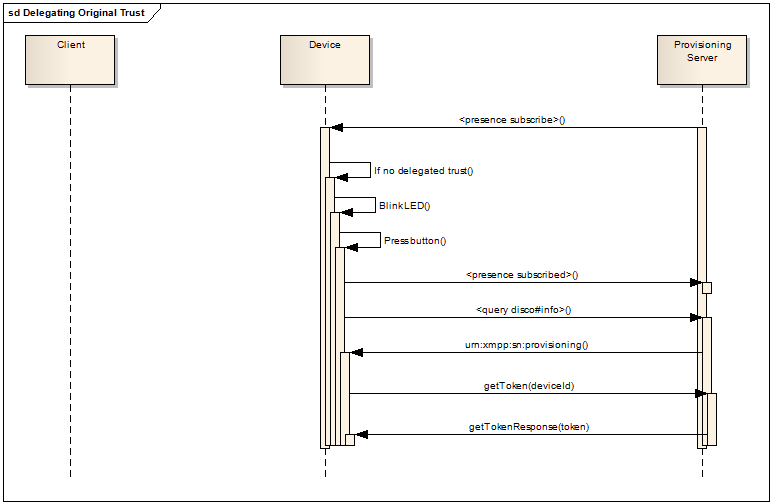
\includegraphics[scale=.25]{images/delegatingTrustSimpleNode}


\subsection{XMPP}

XMPP sends messages using XML streams over a TCP connection. An XML stream is a 
container for the exchange of XML elements between any two entities over 
a network\cite{rfc3920}. To summarize, a TCP connection is established, authenticated, and then bound. The nodes exchange XML stanzas, which is a discrete semantic unit of structured information that is sent from one entity to another over an XML stream. The stream is closed after the exchange, and the TCP connection is closed thereafter.


\subsection{XMPP Related to IoT}

In order for a protocol to support IoT, it must be scalable, secure and simple. Scalability is required due to the large number of nodes involved in connecting all things of the world. A thing can be anything from a light in a house to a vehicle to a trash can. Security is important due to the impact IoT will have on the accessibility of important objects. Simplicity and interoperability come hand in hand due to the diversity of the things involved in IoT.\\
XMPP performs well under a heavy load as exemplified by the observation of public XMPP servers such as MongooseIM. MongooseIM is an XMPP server which performed load tests to find the max number of concurrent users. After 400,000 users were online, memory usage was at 66 percent. It was predicted that 500-600 thousand online users all sending messages would be possible\cite{mongooeIM}. Scalability one of XMPP's strong suits.\\
XMPP supports client authentication and authorization through its XMPP Extension Protocols (XEPs), specifically in XEP-0324: Provisioning. This ensures that the server is properly authenticated and any server certificate properly validated. Devices can be set to only accept control commands from authenticated parties. Security is a focus for XMPP community, which is a necessity for implementing IoT.\\*


\subsubsection{Control}

The Control XEP is a protocol outlining how to set the controllable parameters 
of a node [footnote explaining a node]. The main goal of the Control XEP is 
to make implementation of data setting commands as simple as possible, which is 
fitting for IoT due to the large diversity of the objects that will implement 
the control protocol.\n

XMPP set commands, specifically in the Control XEP, are minimal in implementation. 
The only required fields are the recipient and sender, XML namespace, the name 
and value of the control parameter, and its data type. The XML namespace, line 
3 in Figure 1.1 below, exists to define which protocol is being used to 
exchange data. A sample message from a server to a device is provided below in 
Figure 1.1.\n



\subsubsection{Sensor}

The Sensor Data XEP is a protocol to read the field values that a node [node footnote] may have. The main goals of the Sensor XEP are transparency and compatibility with Control. Since the Sensor Data XEP is the mediator between a client and a node regarding it`s information, Sensor Data is designed to tell the client any and all needed information. Being mediator also implies interaction with the Control XEP, since control exists to set the values of a node.\\
It is important to note the differences between a field value and a control parameter. When the `knobs` of a node are set through the Control XEP, the knobs are the control parameters. When the knobs of a node are being observed through the Sensor Data XEP, the knobs are called fields, by convention. A node`s control parameters are a subset of its fields (which are controllable). The reason for this is that a node may have fields that should not or cannot be set. The Universal Product Code (UPC) of a product is an example of a field that should not be altered. A field may carry a `controllable` flag, but use of this flag is optional. \\
Field values also have slightly different data types than control parameters. The main difference is that Sensor Data has enumeration and numeric data types, which are not available data types in control. The idea behind avoiding enumerations in the Control XEP is that leaving values as strings allows developers the liberty to use units as desired, seeing as a complete set of field names and units is difficult to achieve for any value. However, enums are allowed inside of a device through Sensor Data because XML validation is difficult with free strings and consumers of sensor data need to include unit conversion algorithms. \\
The numeric data type represents a numerical number with an implicit precision and an optional unit. This is for something like temperature...where the numeric variable would be 10 degrees Celsius which is different than 10.0 degrees Celsius in terms of precision. The idea behind avoiding numerics in the Control XEP is that a controller is not assumed to understand how to convert units. \\
Since Sensor Data aims to be completely transparent about a node`s information, a field carries two optional attribute groups. One attribute group is the field`s types which are not to be confused with a fields value types. Field types is a collection of flags that can convey information regarding a specific field that would be useful to a client, such as how long ago the value was set. The flags also include information for if a value can be used for identification, if it`s measured at the time of read-out (or momentary), if it displays status information, if it`s at its peak value, and if it`s computed rather than measured. The other attribute group that a field may carry is it`s quality of service values. These values are also flags that can convey useful information such as the field value not being set, being in progress of measurement, if it`s automatically estimated, whether a warning or error was logged during the measurement period, etc.\\
Like Control, Sensor Data has it`s own version of the getForm command. This is the `all` flag that can be set in a read-out request. This is different than Control in that all fields will be shown, not just those that can be controlled. A sample of this read-out request is above in Figure 2.\\
\begin{figure}
\caption{A sample Sensor Data read-out request}
\lstinputlisting{stanzas/getAll.xml}  
\end{figure}
Since fields have a writable attribute, Sensor Data can be queried to deliver all writeable data. This displays the current control state, just like getForm. Since a node may support both Control and Sensor Data XEPs, it may be holding a value that has a data type that is only included in sensor data. A complete conversion table is laid out in XEP-0325 in this case. The most important mappings are that enums map to strings, and numeric values are simply truncated unless converted to a double (units and precision are lost).\\
A client can also query for specific field types. Especially useful for IoT is the ability to query for momentary values, or values that are measured at run-time of the query. This is useful in that momentary values do not need to be subscribed to, as in a publish/subscribe architecture. The client can simply request a readout of momentary values whenever it feels the need to do so. Clients can optionally set `to` and `from` parameter values, specifying a time range of when the returned values should have been set.\\
Requests always come equipped with the client`s sequence number that requested the data as shown above in Figure 2. Clients pick their sequence number upon their first request. If a request is accepted, the device sends an accepted message and adds the client`s sequence number and request information in a queue. After reading the necessary data, the client then responds with the fields requested if possible, or an error. The client then concludes the interaction with a close message. A use case diagram is in the appendix.


\subsubsection{Provisioning}

The Provisioning XEP is a protocol that focuses on the security aspect of IoT. Provisioning allows the delegation of user privileges and access rights from a provisioning server to the necessary nodes in a network to the users attempting to access them. The main goal of Provisioning is to be implementable for small devices with limited memory and UI options. This relates to IoT because many devices in the network will indeed have limited memory and UI options. \\
The specification for the Provisioning XEP, provides a means of establishing a `trust relationship' between a provisioning server and a sensor with only a single button, LED, and several methods implemented to interact with a provisioning server. The sensor is given a connection to an XMPP server and an id, and the server is notified to create a `presence subscription request' to the sensor. Receiving the first presence subscription request, the sensor flashes its LED and the user installing the sensor presses the button, therefore accepting the request. The sensor now knows of the existence of the provisioning server. The sensor can then query the server to see if it has provisioning implemented. Once it realizes that it does, and that it is communicating with the server, it requests a token to identify itself with for the server. This token is the device's key to accessing methods of other nodes in the network. The sequence diagram, Figure 2.1 below, illustrates the successful case of delegating trust to the provisioning server. \\
\begin{figure*}
\centering
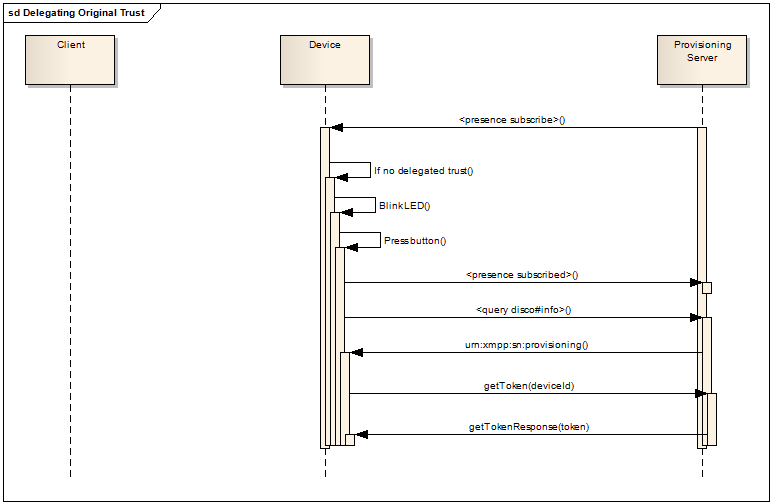
\includegraphics[scale=.5]{images/delegatingTrustSimpleNode}
\caption{Provisioning Server Presence Subscription Request}
\end{figure*}
A token is not solely for the use of a device. Provisioning servers give tokens to services as well, who will use them for set and read commands. Once a provisioning server is installed and running in a network, all devices supporting Control/Sensor Data can be set to require a token if given a command. That way when a service executes a set or read command on a device, its token and command will be passed onto the provisioning server. The server will denote if the given service (and/or human user behind that service) has privileges to run the given command. This is also known as the hasPrivilege query.\\
Since the token is a powerful identification tool, the Provisioning Server has a means of challenging the token to ensure that the device is not spoofing its identity whenever it makes requests using the token. This is possible because the initial call to getToken has a single parameter that is the public part of a Base-64 Public X.509 Certificate. To challenge the device, the provisioning server encrypts a challenge using the public part of the certificate that it received from the original call of getToken and sends the challenge to the device. The device then decrypts the challenge using the private part of the certificate and returns it to the server. \\
Provisioning also has friendships, or the right to send commands to a given device. Upon receiving a presence subscription from a client, a device will ask the provisioning server if the client is its friend. If the server responds with yes, then the device will allow the client to send it commands. If the server responds with no, they have the option to allow the device to add its own friends through a concept called secondary trust.\\
If a device is granted secondary trust, it essentially may converse with anyone that it wishes to. If the device A makes can send commands to other another device B, then essentially any friend that A adds is inherently a friend of B. Due to the unavoidable relationship of the new friend to the B device, XMPP authors warn the reader that secondary trust should be handled with caution.\\


\section{Implementation}

Our initial goal for this project was to implement as many of the IoT XEPs as we
reasonably could, and then to perform Security and Scalability testing and
analysis on our implementation. However, for reasons explained in [SECTION], we
had a fair amount of difficulty getting a good start. Our initial plan was to
implement the Control \& Sensor XEPs, then Provisioning, and finally Concentrator
\& Discovery if we had time.


\subsection{SleekXMPP}

SleekXMPP is an event driven XMPP library developed in python that was used for
implementing the XMPP IoT XEPs. It was one of the few active open implemented
Provisioning in for this project. 


\subsection{Control \& Sensor}

XEPs Control and Sensor were already partially implemented as plugins of the
SleekXMPP library, so we decided to build off of that existing code and to start
developing Provisioning. The existing XEP partial implementations provided us
with a helpful reference when we began to develop Provisioning.

While both the Control and Sensor XEP implementations in SleekXMPP have minimal
functionality, they are both still incomplete. Neither implementation is pep8
compliant, both are confusing for new developers of XMPP IoT, and Control
doesn’t support get forms (See [SECTION] about getforms). We performed a
syntactic cleanup and some slight refactoring of the SleekXMPP code to reduce
these problems.


\subsection{Monkey Wrench in the Sleek Gears}

After spending about a week reading through the SleekXMPP code we began to write
our own implementations of the Control and Sensor XEPs, so that we could compare
it against the SleekXMPP versions. Then we reviewed what parts of implementing
an XEP we needed to understand to begin developing Provisioning.

Before we began coding Provisioning we wrote our own IoT device and console to
exist as proof of concepts of how devices would interact over. The device would
implement a variety of features from Sensor and Control acting as a server (i.e.
not as an XMPP server, but as a device serving sensordata and controllable
fields that a client, in our context the console, would connect to and interact
with). Then we would implement our IoT console, which would act like an end user
application, sending sensordata requests and control commands to affect the
device. Once we had this implemented, we would develop the provisioning
component to then run a provisioning server with Prosody to handle Provisioning
protocol being sent between the IoT console and device.

However we ran into a snag. Once we got our device and console implemented we
were only receiving <service-unavailable> Iq errors. In this context, that meant
that when sending a sensordata request or control command were not listing that
those protocols were being supported in the discovery XEP 0030.

This lead us to believe that some of the features (i.e. a supported XEP/ XMPP
XML namespace)  were not being properly being added to the discovery plugin. We
checked, and as far as we could tell it was properly added. Then we decided to
run their existing discovery browser which gave us the same error but worked
with other common XMPP clients/accounts such as a gmail account logged in with
gchat.

So next we ran the requests locally such that a device would create its own
sensors and request them to itself. This gave us functional result but didn’t
clarify why it wasn’t working to other devices.

We used existing servers xmpp.jp \& darkdna.net, but this left us with
inconsistent results between these two servers; we eventually ran our own server
locally using the Prosody XMPP server.

Then we were finally able to get into contact with Lance (the current maintainer
of SleekXMPP) who was the person who committed Sensor and Control the SleekXMPP.
He was able to help us discover what our problem was. We doing a user error. The
method definition in python specified that the destination jid, source jid, and
asynchronous method callback be put in that order. However we put them in that
order with the pythons definition of position independent parameters (e.g.
\texttt{request\_sensordata(from\_jid= ``jid1'', to\_jid= ``jid2'',
callback=req\_callback})
however it is just supposed to be in that order but without the positional
independent parameter definitions (e.g. request\_sensordata( ``jid1'',  ``jid2'',
req\_callback). This fixed our problem and allowed us to begin development on
Provisioning.

This, while a very simple developer error, eluded us for a variety of reasons.
When we had the initial parameter definitions, SleekXMPP appeared to be doing
what we thought it should be doing. We examined with debug messages and verified
the sent stanza was valid \texttt{request\_sensordata()}. However instead of SleekXMPP
throwing an error locally it sent the packet. Then sleek displayed that we
received an error packet from the device we were sending it to; although
examining the debug logs on the device side it didn’t specify that it was sent
by it. So we aren’t sure if something low level internal to sleekxmpp or the
servers we were using were spoofing a response to our sensordata request with an
error as if it was the device sending it itself.))


\subsection{Console \& Device}

Our IoT console and device were simple proof of concepts to prove that the whole
SleekXMPP stack including XEPs Sensor and Control were functioning so that
Provisioning could be implemented and tested.

The device acts a simple controllable and sensor device that the console can
interact with. Once our provisioning protocol is working these are what we will
extending on top of to utilize the provisioning protocol as clients.


\subsection{Provisioning}

Currently all of the stanza data scructures needed for the Provisioning extended
protocol are in place. We are currently developing what we can of the mechanics
of getting a client and server component of Provisioning to work.

Since there is no XMPP server developed on top of SleekXMPP we had to go with
another server to connect via a server component gateway. This allows us to
continue to develop a functional Provisioning server without having to develop
in any given server’s native language. We decided to be testing and attaching
our Provisioning server component to a Podos server.

What still needs to be done is developing a functional simulated devices
utilizing the Provisioning protocol and the Server component that the devices
will be communicating with to handle the provisioning protocol. Such things
apart of the needed component implementations is attaching the Sleek code to
maintain its state either in memory or in a database for future scalability.
This would maintain friendships, tokens, certificates, etc.


\subsection{Unfinished XEPs}

We had no time to implement or begin the process of implementing a Concentrator
XEP plugin for SleekXMPP or Discovery. Discovery in addition feels a bit to
early in the specification phase to start serious implementation for such open
projects as Sleek.

There is still a lot of work to be done for these extended protocols so that it
can move beyond a proof of concept to testing to see if it meets the actually
minimal goals and needs of IoT protocols such as scalability and security.


\section{Tests}

The only tests were able to run were Unit Tests and running our
IoT console and device locally.

\section{Discussion}

In each of our subsections below we are going to discuss our opinions and
reactions of the IoT XEPs. We will be focusing on how well the Protocols work
for programmers, effectiveness for end users, and thoughts on scalability and
security for each XEP and overall.


\subsection{Developers}

Having different protocols for setting a node`s values and getting a node`s
values can prove to be frustrating for developers. The Control XEP seems to be
the perfect protocol to implement a read request in. Instead, the developer is
forced to support the Sensor Data XEP in order to support readout of meter
values.

Worse yet, the protocols have differences in their view of data types. Sensor
Data has a numeric data type, which is a number with a precision integer and
unit. Control has no concept of the numeric data type, and so the programmer is
forced to implement a default conversion in the sensor if they want the client
to be able to set the numeric data type.

The worst asset to this split up of Control and Sensor data is the
`controllable' flag, which can cause confusion for a user as well, outlined in
the user section below. However, the controllable flag could be turned into a
positive if it were mandatory.

Our solution to the problem of splitting up data fields is that upon giving a
node a data field, the protocol should mandate that the user specify whether the
field is controllable or not through the Sensor Data protocol. That way, Sensor
Data would know the difference between the control parameters (settable) and
fields (only viewable). Essentially, all Sensor Data would need from there is a
set method and Control would cease to serve a purpose.


\subsection{Users}

Having different protocols for setting and getting has a negative effect on the
user due to one particular informational flag that is settable in Sensor Data.
The `controllable` flag, which is optionally set in Sensor Data, indicates
whether a field is settable or not. However, being settable means that the
Control XEP is able to set it, which is defined by behavior in the Control
protocol. So a programmer could make a mistake and mark a certain field as
`settable` through the Sensor Data protocol, when it all reality Control cannot
even touch it. This could cause lots of confusion for a user that wishes to view
control parameters through the read command of Sensor Data rather than the
getForm command of Control.

Provisioning only has a notion of access rights for individual friends and
doesn't allow for groupings. This prevents group properties or means of group
relationships which may result in more work for managing trust relationships for
end users than effectively necessary.


\subsection{Security}

Approach taken as a protocol should be one of that assume devices, services, and
servers not only exist in an unreliable network but an actively malicious one.
Also it may be arguable that there may be no IoT protocol like IPv4 there is for
the Internet. It may from the beginning need to find a commonality among current
protocols to see what minimum features exist amongst all of them and not only
try to provide the best protocol can for their own purposes but assume that
gateways will be able to exist or devices may need to speak multiple IoT
protocols to function in the world around them. 

Provisioning chain of trust. Strange that a spec doesn`t clarify that a device
or user can send an unfriend request. The provisioning server is the only one
who makes that decision.

Provisioning The protocol currently specifies that if there are multiple
provisioning servers on the that are returning access rights (e.g.  CanRead,
CanAccess, CanControl), a device is supposed to apply a Union operation to these
provisioning server responses. This results in a design of potential fail
opening.

Example then is if a company has multiple of provisioning servers for
redundancy and handling larger networks. It doesn`t take the effort of
compromising all of the provisioning servers to abuse the rights of a
device. If you have control of one provisioning server you can override what
may be the valid access controls of all of the other provisioning servers.

Provisioning Authentication. One weakness in authentication of devices,
apart of the XMPP IoT network, is that they only send requests to a service
requesting tokens, which is then delegated between the service and
provisioning server to update or manage the access and controls. The
authentication relies on the SASL and TLS authentication below it and
doesn`t really provide any new level of authentication on the overly IoT
network. It seems to be unclear if the SASL and TLS are sufficient
authentication for devices on a network.`


\section{Conclusion}

In the paper we explain the current of the basal IoT protocols for XMPP and
our critique of them through the process of trying to implement the
Provisioning XEP. The protocol is no were near complete and needs several
attempts of implementation and refactoring of the protocol to become a
usable protocol in the future.


\nocite{*}
\bibliographystyle{IEEEannot}
\bibliography{citations}

\clearpage
\newpage

\onecolumn
\appendix
\section{Control Get Form}
\label{appendix_a}

\lstinputlisting[language=XML,
                 numbers=left,
                 breaklines=true,
                 stepnumber=1]{stanzas/getForm.xml}

\end{document}
